\chapter{Extended Operators and Topological Defects}
\label{ch:extended-operators-topological-defects}

\ConventionsMixed

Extended operators are QFT data supported on submanifolds.  Their definition
fixes allowed singularities, endpoint conditions, defect degrees of freedom,
counterterms along the support, and the correlation functionals obtained after
the regulator is removed.  Local operator algebras control the behavior near
points.  A full theory also contains a completion by line, surface, wall, and
higher-codimension objects, together with rules for their collision, crossing,
and fusion.

\section{Submanifold Support And Tubular Neighborhood Data}

Let \(M\) be a smooth \(D\)-dimensional spacetime manifold, Euclidean or
Lorentzian according to the context.  Let
\[
  i:\Sigma^p\hookrightarrow M
\]
be a properly embedded oriented \(p\)-manifold.  Its normal bundle is
\[
  N_{\Sigma/M}=i^*TM/T\Sigma ,
  \qquad
  \operatorname{rank}N_{\Sigma/M}=D-p .
\]
When a framing, spin structure, orientation of the normal bundle, or
background gauge field is required, that structure is part of the support
datum.  For sufficiently small \(\varepsilon>0\), a tubular neighborhood is a
disk bundle
\[
  T_\varepsilon(\Sigma)\subset N_{\Sigma/M}
\]
embedded in \(M\).  The punctured neighborhood
\[
  T_\varepsilon(\Sigma)\setminus\Sigma
\]
records how bulk fields approach the support.

\begin{definition}[Extended operator datum]
\label{def:extended-operator-datum}
An extended operator \(D(\Sigma)\) supported on \(\Sigma\subset M\) is a
renormalized correlation-functional datum consisting of:
\[
\begin{array}{ll}
  \text{support data} &
  (\Sigma,N_{\Sigma/M})\text{ with the declared auxiliary structures},\\[1mm]
  \text{bulk condition} &
  \text{allowed fields on }M\setminus T_\varepsilon(\Sigma),\\[1mm]
  \text{normal model} &
  \text{singular or boundary behavior on }\partial T_\varepsilon(\Sigma),\\[1mm]
  \text{defect fields} &
  \text{degrees of freedom living on }\Sigma\text{ when present},\\[1mm]
  \text{coupling} &
  \text{local terms coupling bulk and defect variables},\\[1mm]
  \text{counterterms} &
  \text{local functionals on }\Sigma\text{ used in the limit }\varepsilon\to0,\\[1mm]
  \text{correlators} &
  \text{distributions with insertions away from }\Sigma .
\end{array}
\]
Two representatives define the same extended operator when all renormalized
correlation distributions with external insertions away from the support
agree.
\end{definition}

For local fields \(\mathcal O_j(x_j)\) inserted at points
\[
  x_j\in M\setminus\Sigma ,
\]
the defining distributions are
\[
  \left\langle
    D(\Sigma)\,\mathcal O_1(x_1)\cdots\mathcal O_n(x_n)
  \right\rangle .
\]
They are defined on the configuration space where the \(x_j\) are pairwise
distinct and avoid \(\Sigma\), and they are extended to collision loci by a
chosen bulk and defect renormalization prescription.  The bulk-to-defect
operator product expansion is the local expansion, in a normal coordinate
\[
  x=\exp_y(r\hat n),\qquad y\in\Sigma,\quad \hat n\in S(N_{\Sigma/M,y}),
\]
of a bulk operator near the defect:
\[
  \mathcal O(x)\,D(\Sigma)
  \sim
  \sum_\alpha C_{\mathcal O\alpha}(r,\hat n;\partial_y)\,
  \widehat{\mathcal O}_\alpha(y)\,D(\Sigma).
\]
The operators \(\widehat{\mathcal O}_\alpha\) are local operators of the
defect theory on \(\Sigma\).  The coefficients are distributions in the
normal variables and differential operators along \(\Sigma\).  This expansion
is part of the defect's short-distance data, just as the ordinary OPE is part
of the local operator algebra.

Figure~\ref{fig:extended-defect-basic-operations} records the basic operations
on extended defects used in this chapter: tubular neighborhoods, defect-local
operators, fusion, and deformation through topological regions.

\begin{figure}[H]
\centering
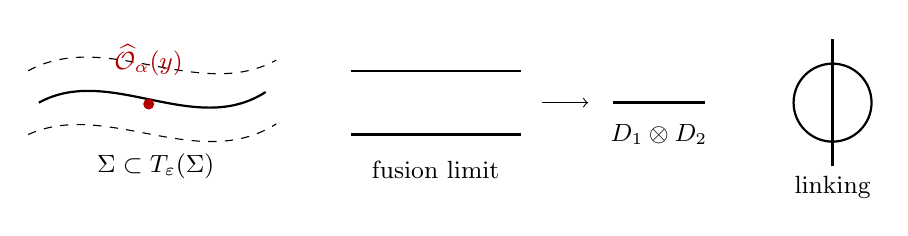
\begin{tikzpicture}[scale=0.9, every node/.style={font=\small}]
  \draw[thick] (-0.2,0) .. controls (0.8,0.55) and (2.0,-0.5) .. (3.0,0.15);
  \draw[dashed] (-0.35,0.45) .. controls (0.75,1.05) and (2.05,0.0) .. (3.15,0.6);
  \draw[dashed] (-0.35,-0.45) .. controls (0.75,0.05) and (2.05,-1.0) .. (3.15,-0.3);
  \fill[red!70!black] (1.35,-0.02) circle (2.2pt);
  \node[red!70!black,above] at (1.35,0.24) {\(\widehat{\mathcal O}_\alpha(y)\)};
  \node at (1.45,-0.9) {\(\Sigma\subset T_\varepsilon(\Sigma)\)};

  \draw[thick] (4.2,0.45) -- (6.6,0.45);
  \draw[thick] (4.2,-0.45) -- (6.6,-0.45);
  \draw[->] (6.9,0) -- (7.55,0);
  \draw[very thick] (7.9,0) -- (9.2,0);
  \node at (5.4,-0.95) {fusion limit};
  \node at (8.55,-0.45) {\(D_1\otimes D_2\)};

  \draw[thick] (11.0,0) circle (0.55);
  \draw[very thick] (11.0,-0.9) -- (11.0,0.9);
  \node at (11.0,-1.2) {linking};
\end{tikzpicture}
\caption{Tubular-neighborhood data for a defect \(\Sigma\), including a
defect-local insertion \(\widehat{\mathcal O}_\alpha(y)\), fusion of parallel
defects, and a topological linking configuration.}
\label{fig:extended-defect-basic-operations}
\end{figure}

\section{Genuine Defects, Boundaries, And Junctions}

Let \(D(\Sigma)\) have codimension \(c=D-p\).  A defect is genuine when its
definition uses only data on an arbitrarily small tubular neighborhood of
\(\Sigma\) and the complement \(M\setminus\Sigma\).  If an additional
\((p+1)\)-dimensional submanifold \(B\) with
\[
  \partial B=\Sigma
\]
is required, then the insertion is a boundary of a higher defect rather than
an autonomous \(p\)-dimensional defect.  This distinction is part of the
operator spectrum of the theory.

If two \(p\)-dimensional defects \(D_a\) and \(D_b\) meet along a
\((p-1)\)-dimensional submanifold \(J\), the junction is a lower-dimensional
defect operator
\[
  \Psi_{ab}(J)\in\operatorname{Hom}(D_a,D_b)
\]
in the defect category appropriate to the theory.  For a line operator, a
point endpoint is a local operator in such a Hom space.  In gauge theory, a
Wilson line in representation \(R\) ending at a point requires an endpoint
operator transforming in \(R^\vee\) or an equivalent charged state.  The
existence of such an endpoint is the operator statement of screening.

\section{The Displacement Operator}

Let \(D(\Sigma)\) be a renormalized defect in a QFT with stress tensor
\(T_{\mu\nu}\).  Near a point of \(\Sigma\), choose coordinates
\[
  (y^a,n^i),\qquad
  a=1,\ldots,p,\quad i=1,\ldots,D-p,
\]
where \(y^a\) are tangent to \(\Sigma\) and \(n^i\) are normal coordinates.
Translation perpendicular to the defect is broken by the insertion.  The
corresponding Ward identity has the form
\[
  \nabla_\mu T^{\mu i}(y,n)
  =
  \delta_\Sigma(n)\,\mathcal D^i(y)
\]
inside correlation functions with the defect inserted, up to contact terms
with other insertions.  The defect local operator
\[
  \mathcal D^i(y)
\]
is the displacement operator.  Its index is a section of
\[
  N_{\Sigma/M}.
\]
The identity is a definition of the normalization of \(\mathcal D^i\).

\begin{proposition}[Shape variation and displacement]
\label{prop:shape-variation-displacement}
Let \(\Sigma_t\) be a smooth one-parameter family of embedded supports with
\(\Sigma_0=\Sigma\).  Let
\[
  v^i(y)=\left.\frac{d\Sigma_t}{dt}\right|_{t=0}
\]
be the normal deformation vector.  Assume the external insertions are kept
away from the swept tubular neighborhood and that no boundary term is produced
at infinity or at \(\partial\Sigma\).  Then
\[
  \left.\frac{d}{dt}\right|_{t=0}
  \left\langle D(\Sigma_t)\,\mathcal X\right\rangle
  =
  -\int_\Sigma d^py\,\sqrt{h}\,
  v_i(y)
  \left\langle
    \mathcal D^i(y)\,D(\Sigma)\,\mathcal X
  \right\rangle ,
\]
where \(h\) is the induced metric on \(\Sigma\) and \(\mathcal X\) is the
product of external insertions.
\end{proposition}

\begin{proof}
Represent the deformation by a diffeomorphism generated by a vector field
\(v^\mu\) supported in the tubular neighborhood and normal to \(\Sigma\) on
the support.  The variation of a correlation functional under this
diffeomorphism is the Ward variation generated by the stress tensor:
\[
  \delta_v\langle D(\Sigma)\mathcal X\rangle
  =
  -\int_M d^Dx\,\sqrt{g}\,
  \nabla_\mu v_\nu
  \langle T^{\mu\nu}(x)D(\Sigma)\mathcal X\rangle .
\]
Integrating by parts gives
\[
  \delta_v\langle D(\Sigma)\mathcal X\rangle
  =
  \int_M d^Dx\,\sqrt{g}\,
  v_\nu
  \langle\nabla_\mu T^{\mu\nu}(x)D(\Sigma)\mathcal X\rangle ,
\]
with no boundary contribution by hypothesis.  Tangential components generate
reparametrizations of the support, so only the normal components contribute
to the shape.  Inserting the defect Ward identity
\[
  \nabla_\mu T^{\mu i}=\delta_\Sigma\mathcal D^i
\]
and using
\[
  \int_M d^Dx\,\sqrt{g}\,\delta_\Sigma(n)f(x)
  =
  \int_\Sigma d^py\,\sqrt h\,f(y,0)
\]
gives the stated formula, with the sign fixed by the convention that moving
the support rather than the coordinates gives the opposite diffeomorphism.
\end{proof}

\begin{definition}[Topological defect]
\label{def:topological-defect}
A defect \(D(\Sigma)\) is topological relative to a declared class of
background structures when its renormalized correlation functionals are
invariant under every isotopy of \(\Sigma\) that preserves those background
structures and avoids the other insertions.
\end{definition}

\paragraph{Displacement criterion.}
Under the hypotheses of Proposition~\ref{prop:shape-variation-displacement},
if the displacement operator vanishes inside the physical correlation
functionals, then \(D(\Sigma)\) is topological.  In a cohomological theory
with odd differential \(Q\), the same conclusion holds for \(Q\)-closed
external insertions when
\[
  \mathcal D^i=\{Q,\mathcal V^i\}_{\mathrm{gr}}
\]
and the \(Q\)-Ward identity has no boundary contribution.

The shape derivative is the integral of the displacement insertion.  If the
displacement insertion vanishes in all relevant correlators, the derivative
along every isotopy path is zero.  If
\(\mathcal D^i=\{Q,\mathcal V^i\}_{\mathrm{gr}}\), the integrand is a
\(Q\)-variation after moving \(Q\) through the \(Q\)-closed external
insertions.  The Ward identity sets the expectation value of this
\(Q\)-variation to zero.  Hence the correlation functional is constant along
the isotopy.

\section{Fusion}

Let \(D_1(\Sigma)\) and \(D_2(\Sigma)\) be topological defects of the same
dimension and compatible normal structures.  Choose two nearby parallel
copies \(\Sigma_0,\Sigma_\varepsilon\) inside a tubular neighborhood.  Their
fusion is defined by the correlation-function limit
\[
  (D_1\otimes D_2)(\Sigma)
  =
  \lim_{\varepsilon\downarrow0}
  D_1(\Sigma_\varepsilon)D_2(\Sigma_0),
\]
with external insertions kept outside the tubular neighborhood.  The limit is
taken after subtracting local defect counterterms supported on \(\Sigma\).
The result can be a single defect, a finite direct sum, an integral over
continuous labels, or a distributional kernel.  The precise target depends on
the analytic category in which the QFT and its defects are defined.

Fusion is associative when the triple-collision limits are compatible:
\[
  (D_1\otimes D_2)\otimes D_3
  \cong
  D_1\otimes(D_2\otimes D_3).
\]
The isomorphism is part of the defect data.  In a fully extended topological
theory these associators, unit defects, adjoints, and higher junctions form a
higher category.  In a non-topological QFT, the same language applies only to
the topological subsector of defects or to protected cohomological defects
for which the required collision limits exist.

\begin{example}[Group-like topological defects]
\label{ex:group-like-topological-defects}
Let \(A\) be a finite abelian group.  A set of invertible topological defects
\[
  \{U_a\}_{a\in A}
\]
is group-like when
\[
  U_a\otimes U_b=U_{a+b},
  \qquad
  U_0=\mathbf 1,
  \qquad
  U_a^{-1}=U_{-a}.
\]
For \(A=\mathbb Z_N\), this says
\[
  U_r\otimes U_s=U_{r+s\ {\rm mod}\ N}.
\]
The associator may be trivial or may carry a cocycle.  A nontrivial cocycle
is part of the anomaly data of the symmetry-defect system.
\end{example}

\section{Higher-Form Ward Defects}

Let \(A\) be an abelian \(p\)-form symmetry group in a \(D\)-dimensional QFT.
For
\[
  a\in A
\]
there is a topological symmetry defect
\[
  U_a(N)
\]
supported on an oriented closed \((D-p-1)\)-manifold
\[
  N^{D-p-1}\subset M .
\]
A charged \(p\)-dimensional operator
\[
  W_q(\Sigma^p)
\]
has charge
\[
  q\in\widehat A=\operatorname{Hom}(A,U(1)).
\]
There is a canonical integer linking coordinate in the local chart used for
Ward identities.  Namely, if the isotopy is contained in a ball, or if
\(M=\mathbb R^D\) with compact supports, equivalently \(S^D\) after
one-point compactification, then a closed symmetry-defect support \(N\)
disjoint from \(\Sigma\) has an integer
\[
  \operatorname{Link}_{\rm loc}(N,\Sigma)\in\mathbb Z .
\]
If \(N=\partial B\) for an oriented \((D-p)\)-chain \(B\) transverse to
\(\Sigma\), this integer is
\[
  \operatorname{Link}_{\rm loc}(N,\Sigma)=B\cdot\Sigma ,
\]
the signed intersection number.  In these local or spherical settings this is
the Alexander-duality coordinate of the class of \(N\) in the complement of
\(\Sigma\).

On a general spacetime manifold \(M\), the same displayed intersection formula
is a controlled chart only after extra topology is declared.  First,
\(N\) must bound such a chain \(B\).  Second, the value must be independent of
the chosen bounding chain: if \(B'\) is another choice, the ambiguity is
\[
  (B-B')\cdot\Sigma ,
\]
with \(B-B'\) a closed \((D-p)\)-cycle.  Thus independence holds, for example,
when the homology class of \(\Sigma\) pairs trivially with
\(H_{D-p}(M;\mathbb Z)\).  If \(N\) does not bound, or if this ambiguity
survives, an integer \(B\cdot\Sigma\) is additional bounding-chain data rather
than a canonical global linking number.

There are two standard global replacements, but their degrees must be kept
separate.  The characteristic class of a finite \(p\)-form background is
\[
  [B]\in H^{p+1}(M;A).
\]
This class evaluates on \((p+1)\)-cycles; it is not itself a functional on the
\(p\)-cycle \([\Sigma]\).  To write the phase of \(W_q(\Sigma)\), one must
choose the operator holonomy data: for example a cochain or
differential-cohomology representative \(\check B\) with a declared
\(p\)-cycle holonomy
\[
  \operatorname{Hol}_{\check B}(\Sigma)\in A,
  \qquad
  W_q(\Sigma)\mapsto
  q\!\left(\operatorname{Hol}_{\check B}(\Sigma)\right)W_q(\Sigma),
\]
or, for an ordinary symmetry transformation, a degree-\(p\) gauge parameter
\(\lambda\in Z^p(M;A)\) with \(B\mapsto B+\delta\lambda\), acting by
\[
  W_q(\Sigma)\mapsto
  q\!\left(\langle\lambda,[\Sigma]\rangle\right)W_q(\Sigma).
\]
A codimension-\((p+1)\) symmetry defect is typed similarly: its relative or
Thom class is degree \(p+1\), and a specified transgression, slant, cap, or
bounding-chain construction produces the degree-\(p\) complement datum that is
evaluated on \(\Sigma\).  In the local chart this transgressed datum is exactly
the integer-linking phase above.
For torsion supports on a closed oriented manifold, the global linking datum is
the torsion pairing
\[
  \lambda_{\rm tor}:
  \operatorname{Tor}H_{D-p-1}(M;\mathbb Z)
  \times
  \operatorname{Tor}H_p(M;\mathbb Z)
  \longrightarrow
  \mathbb Q/\mathbb Z ,
\]
which a finite character can exponentiate.  It is a \(\mathbb Q/\mathbb Z\)
coordinate, not an integer intersection number.

\paragraph{Higher-form Ward action.}
In the local integer-linking chart, an abelian \(p\)-form symmetry defect
\(U_a(N)\) and a charged \(p\)-operator \(W_q(\Sigma)\) obey the Ward action
\[
  U_a(N)\,W_q(\Sigma)
  =
  q(a)^{\operatorname{Link}_{\rm loc}(N,\Sigma)}
  W_q(\Sigma)
\]
inside correlation functions whose other insertions are outside the isotopy
region.  For \(A=\mathbb Z_N\), with \(a=r\) and \(q=s\) represented by
integers modulo \(N\),
\[
  q(a)=\exp\left(\frac{2\pi i\,rs}{N}\right).
\]
This is the topological definition of the local action written in
linking-number form.  Because \(U_a\) is topological, move \(N\) through the
complement of \(\Sigma\) without changing the correlator.  The only change
occurs when the swept chain crosses \(\Sigma\).  A single positive crossing
implements the symmetry action on \(W_q\), which is multiplication by the
character
\[
  q(a)\in U(1).
\]
A negative crossing contributes \(q(a)^{-1}\).  Summing the signed crossings
gives the intersection number \(B\cdot\Sigma\) for a bounding chain
\(\partial B=N\) in the local chart, or in a global chart where the
bounding-chain ambiguity vanishes.  On nontrivial \(M\), a wrapping symmetry
defect is evaluated by the chosen holonomy/transgression or torsion-pairing
datum above.
For \(\mathbb Z_N\), the character group is canonically \(\mathbb Z_N\) after
choosing the generator
\[
s(r)=\exp(2\pi i\,rs/N),
\]
which gives the displayed phase.

The dimensions satisfy
\[
  \dim N+\dim\Sigma=(D-p-1)+p=D-1,
\]
which is the dimension condition for linking in \(D\) dimensions.  If
\(N\) crosses an endpoint or junction of \(W_q\), the Ward identity includes
the action on that endpoint or junction operator as well.  Charge
conservation at a junction is the statement that the product of all character
factors associated with a small linking symmetry defect around the junction
is one.

\section{Locality And Braiding}

In Lorentzian signature, two extended operators with spacelike separated
supports admit an exchange operation.  For ordinary bosonic local operators
this exchange is commutation.  For line, surface, and defect operators the
exchange can carry a braiding determined by topology, spin, and gauge charge.
The braiding is measured by transporting one support around another in the
configuration space of disjoint submanifolds.

For abelian Wilson--'t Hooft line charges
\[
  \gamma=(\lambda,m),
  \qquad
  \gamma'=(\lambda',m'),
\]
the center-sensitive part of the braiding phase is
\[
  \exp\bigl(2\pi i\,B(\gamma,\gamma')\bigr),
  \qquad
  B(\gamma,\gamma')=\lambda(m')-\lambda'(m),
\]
with the pairing defined in
Chapter~\ref{ch:global-forms-higher-form-symmetry}.  A line spectrum in a
four-dimensional gauge theory is mutually local when this phase is one for
every pair of genuine lines in the declared spectrum.  The analytic
construction of the corresponding magnetic and dyonic lines is developed in
Chapter~\ref{ch:global-line-surface-domain-wall-operators}.

\section{Defect Completeness Data}

The local observable net or Wightman field content determines many
constraints on defects: covariance, locality, stress-tensor Ward identities,
superselection sectors, and possible endpoint charges.  A QFT also contains
additional completion data specifying which extended operators are genuine,
which higher defects they may bound, which junctions exist, and which fusion
limits are part of the theory.  Distinct global forms of a gauge theory have
the same local Lie algebra and perturbative local vertices but different
line spectra and higher-form symmetry defects.  This is the basic reason that
extended operators must be included as primary QFT data in any complete
nonperturbative definition.

\begin{openproblem}[Extended operators from local reconstruction]
\label{op:extended-operators-from-local-reconstruction}
Develop reconstruction theorems that recover the extended-operator
completion of a QFT from local observables, phase-space or split-property
data, superselection sectors, and specified global-form input.  The target
is a theorem that identifies the genuine line, surface, wall, endpoint,
junction, and fusion data determined by locality and duality, and separates
that determined part from additional global completion choices.
\end{openproblem}
